\section{Compiler}
\labsec{ch04-compiler}

Our second main goal is to design an implement a compiler for our syntax such that
it provides parsing a source file, \textbf{sintactic} and \textbf{semantic} validation,
warnings and errors emition and code generation.

Upon this point we know that the target that we want our compiler to produce is not a binary
nor any similar executable file. But instead we will develop a feature to translate the
schemas on to object-oriented domain models. For this reason this section will only analyse
what it is called the front-end \sidecite{levy1998compiler} of the compiler and next section
will be devoted to the code generation feature (compiler back-end).

Also as the compiler itself represents a piece of software we will analyse its target users,
the different use cases for each profile and finally the requirements that the compiler, as
a system, must meet.

\subsection{Target Users}
Every system has some target users, in the case of the ShEx-Lite compiler we will focus it on three different types of users:
\begin{itemize}
    \item \textbf{People with low technical skills} that want to make schemas to validate RDF by means
    of shape expressions. This people will be able to compile their schemes and check for
    syntax / semantic errors or warnings through the CLI with a very simple instruction set.
    \item \textbf{People with medium technical skills} that want to make schemas to validate RDF by means
    of shape expressions. This people will be able to compile their schemes and check for
    syntax / semantic errors or warnings through an API.
    \item \textbf{ShEx Community developers} that want to test a new feature by implementing and
    testing its behaviors in a controlled small environment. For this people the compiler
    provides not only the public API but the source code and the corresponding technical
    documentation. 
\end{itemize}

\subsection{Use Cases}
The first stage to analyze our system is to see the use cases view, from there we will try to capture
posible requirements and with all that information design our system.

\begin{figure}[hb]
    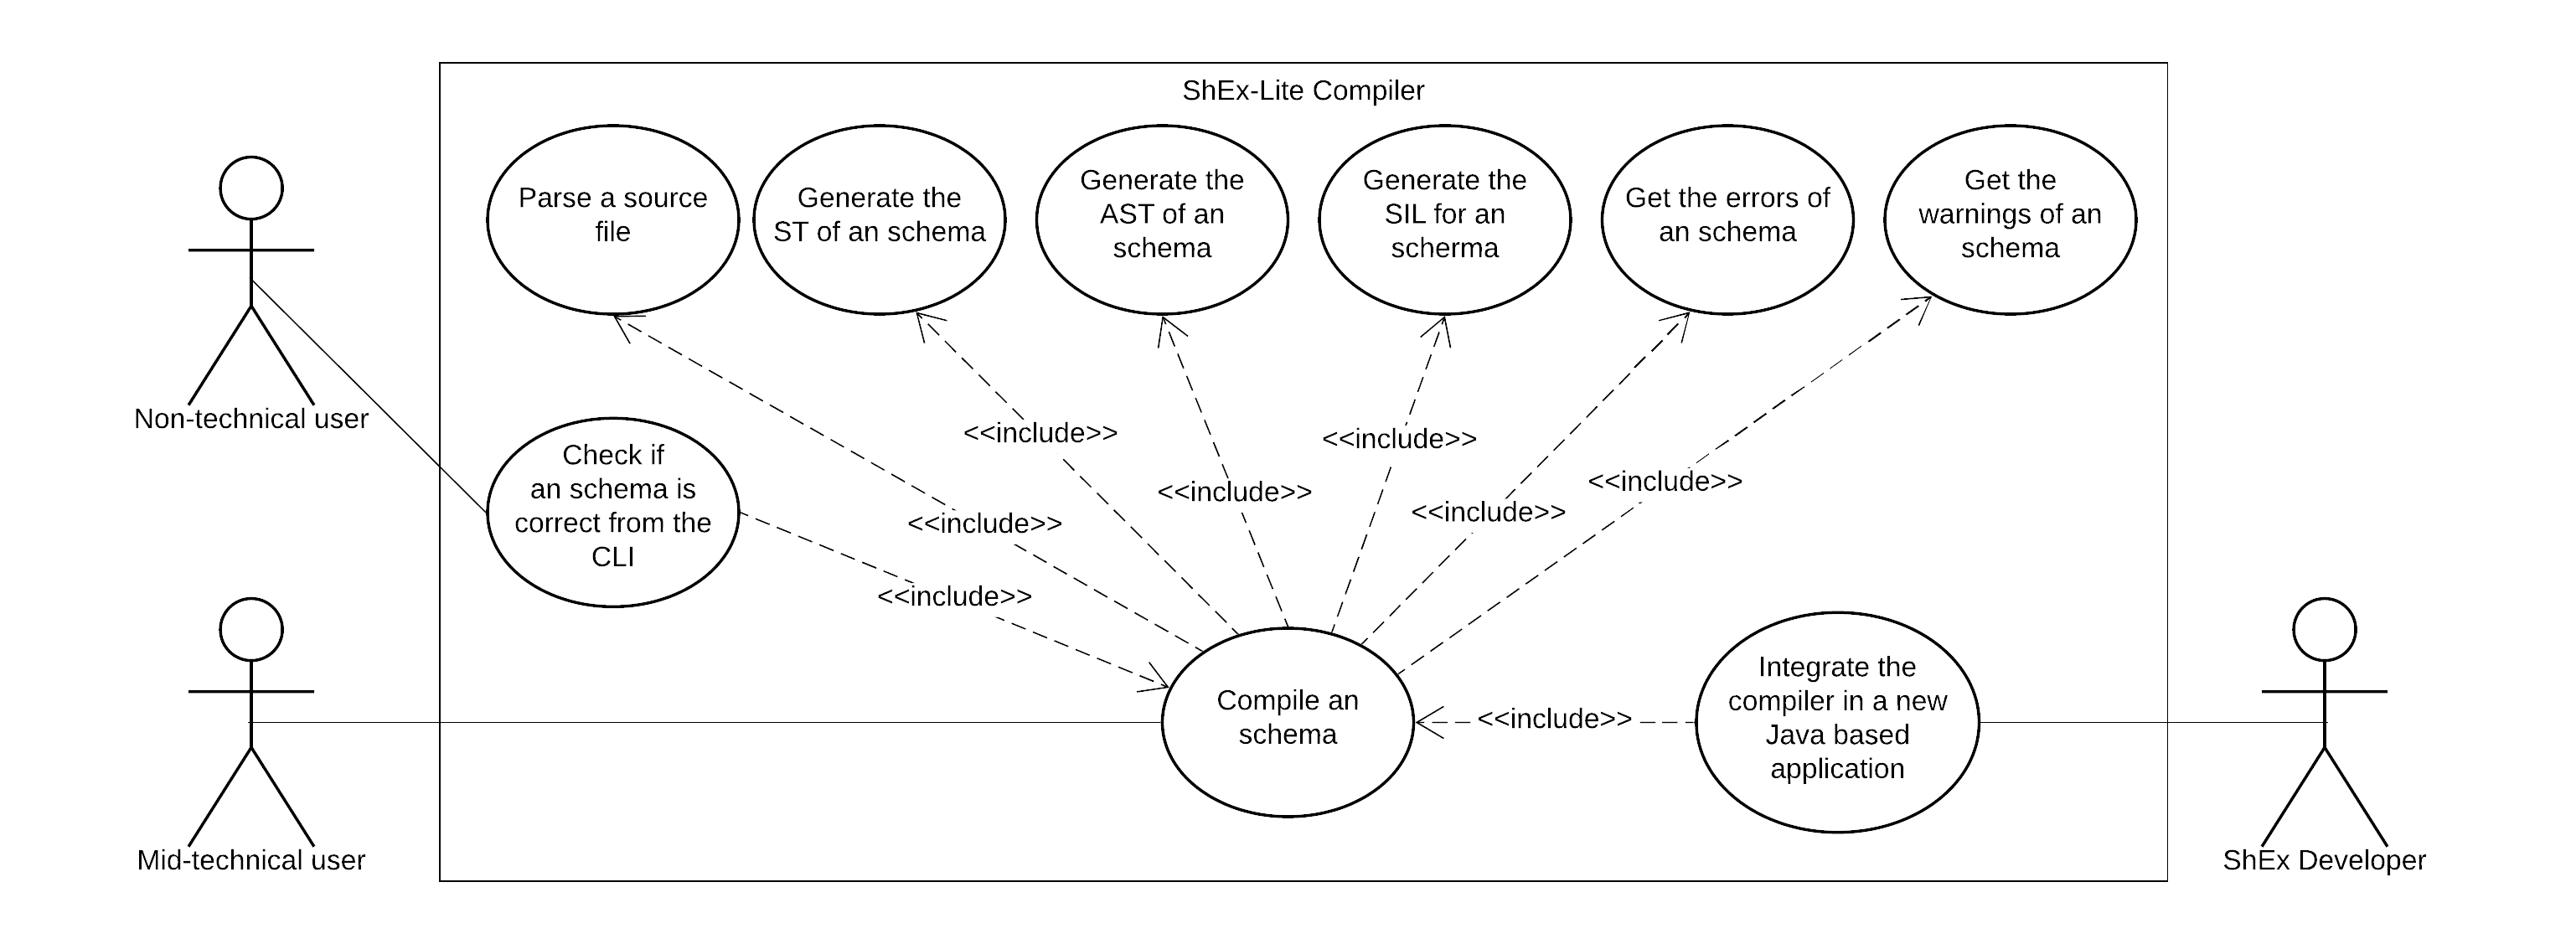
\includegraphics{shex-lite-compiler-use-case-general.png}
    \caption[Use cases view of the ShEx-Lite compiler for the three different 
    actors of the system]{Use cases view of the ShEx-Lite compiler for the three different actors of the system.}
    \labfig{shex-lite-use-cases-01}
\end{figure}

In \reffig{shex-lite-use-cases-01} we can see the high level view of the different use cases that 
the three different target users of the systems might have, now we will analyze each one individually,
some the internal use cases that have no direct interaction with the target user will be explored after.

\subsubsection{Non technical user}
The non technical target user is intended to use only the compiler to validate if the schemas they
have defined are syntactically and semantically correct. And if they have any error or warning to be
aware of them. \reffig{shex-lite-use-cases-02} shows the interaction diagram for this actor, and
\reftab{use-case-01-tab} describes the represented use case.

\begin{figure}[hb]
    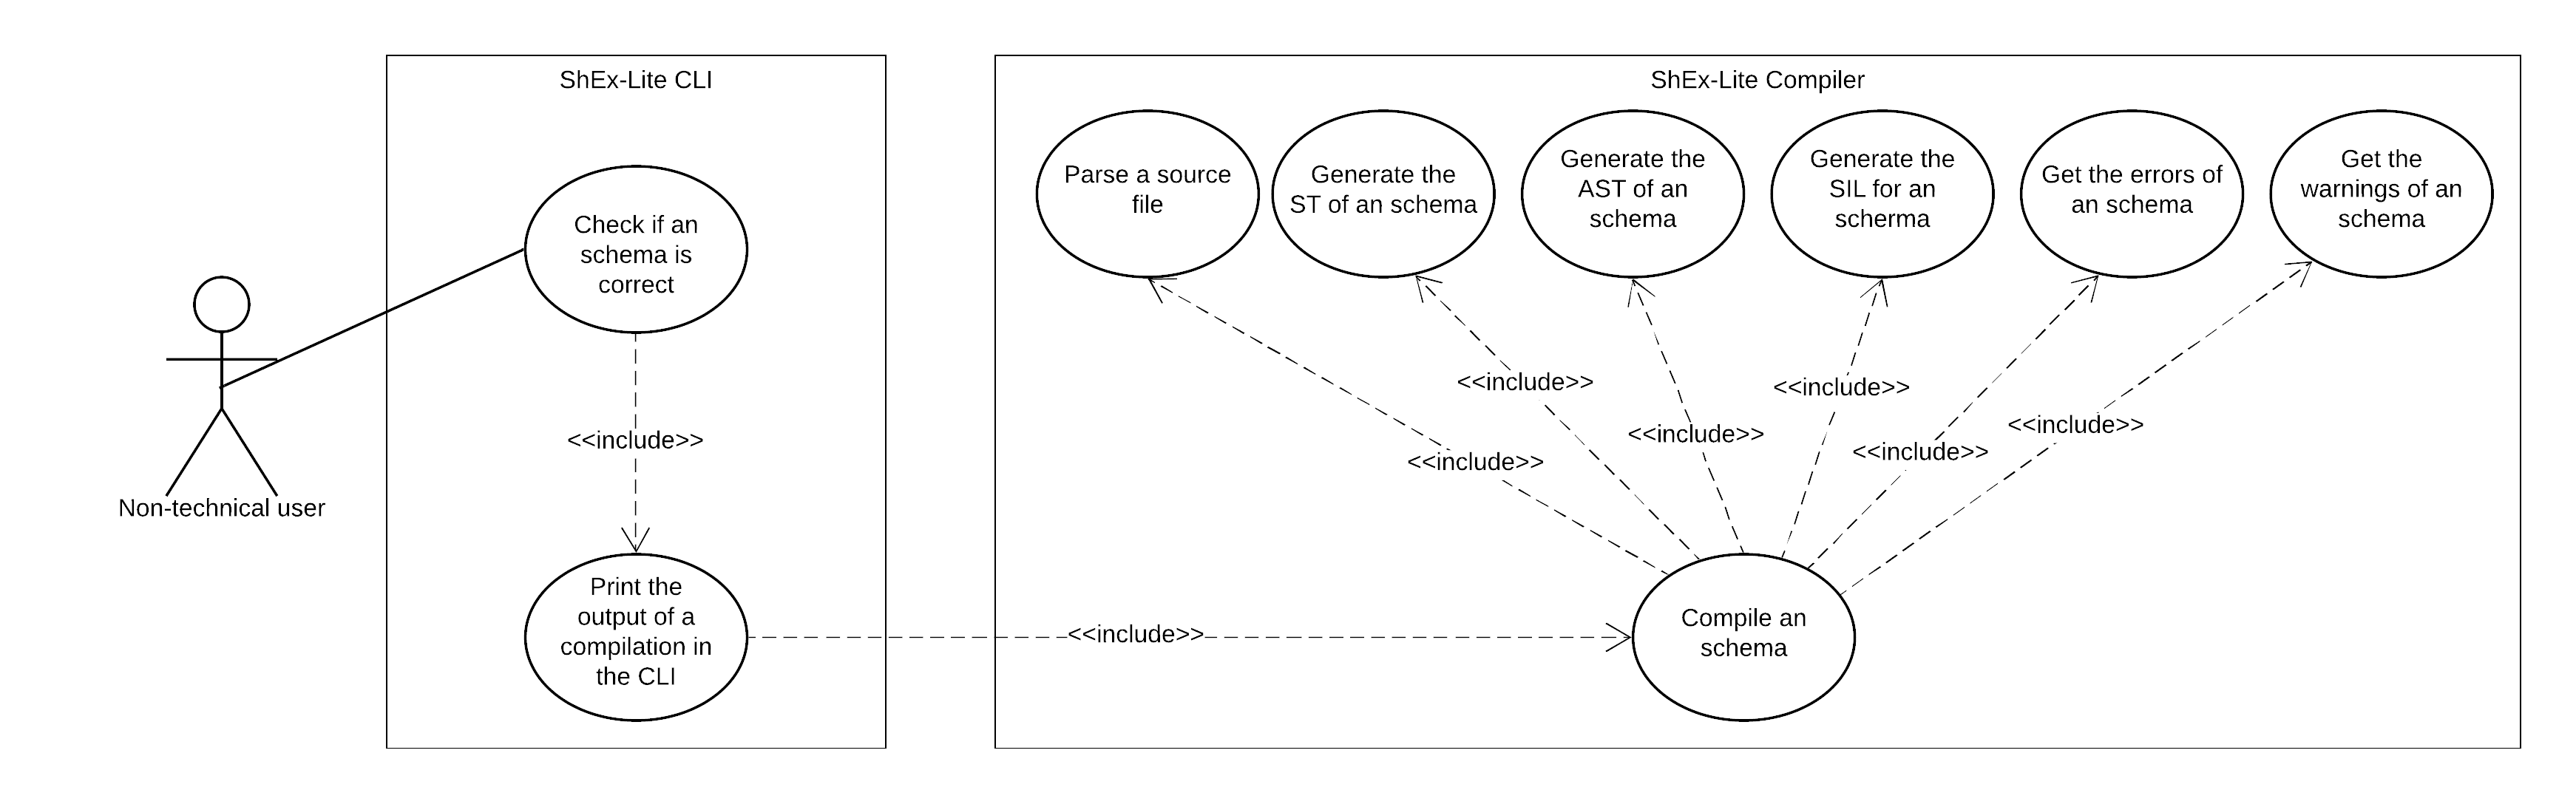
\includegraphics{shex-lite-use-cases-02.png}
    \caption[Extension of the use case view for a non technical user]{Extension of the use 
    case view for a non technical user.}
    \labfig{shex-lite-use-cases-02}
\end{figure}

\begin{table}[hb]
    \begin{tabular}{ | m{2cm} | m{8cm}| }
        \hline
        Use Case Number & 1 \\
        \hline
        Description & Check if an schema is correct from the CLI tool. \\
        \hline
        Actor & Non technical user. \\
        \hline
        Flow & The actor wants to check if schema is correct or not. If it is not correct wants to see all 
        the warnings / errors. For this purpose the actor introduces the schema in the CLI tool and starts 
        the flow. Once the flow is complete the actor wants to see information that helps to decide if the 
        schema is correct or not. \\
        \hline
    \end{tabular}
    \caption[Definition of the use case number 1 for the non technical user]{Definition of the use case number 
    1 for the non technical user.}
    \labtab{use-case-01-tab}
\end{table}

\subsubsection{Mid technical user}
For the mid technicas user, from \reffig{shex-lite-use-cases-01}, we see that the use case is very similar to the
one of the user with low technical skills but with one difference. This profile wants to validate schemas by using
the API. For this profile we can find the representation of the interaction diagram at \reffig{shex-lite-use-cases-03}
and the associated use case description on \reftab{use-case-02-tab}.

\begin{figure}[hb]
    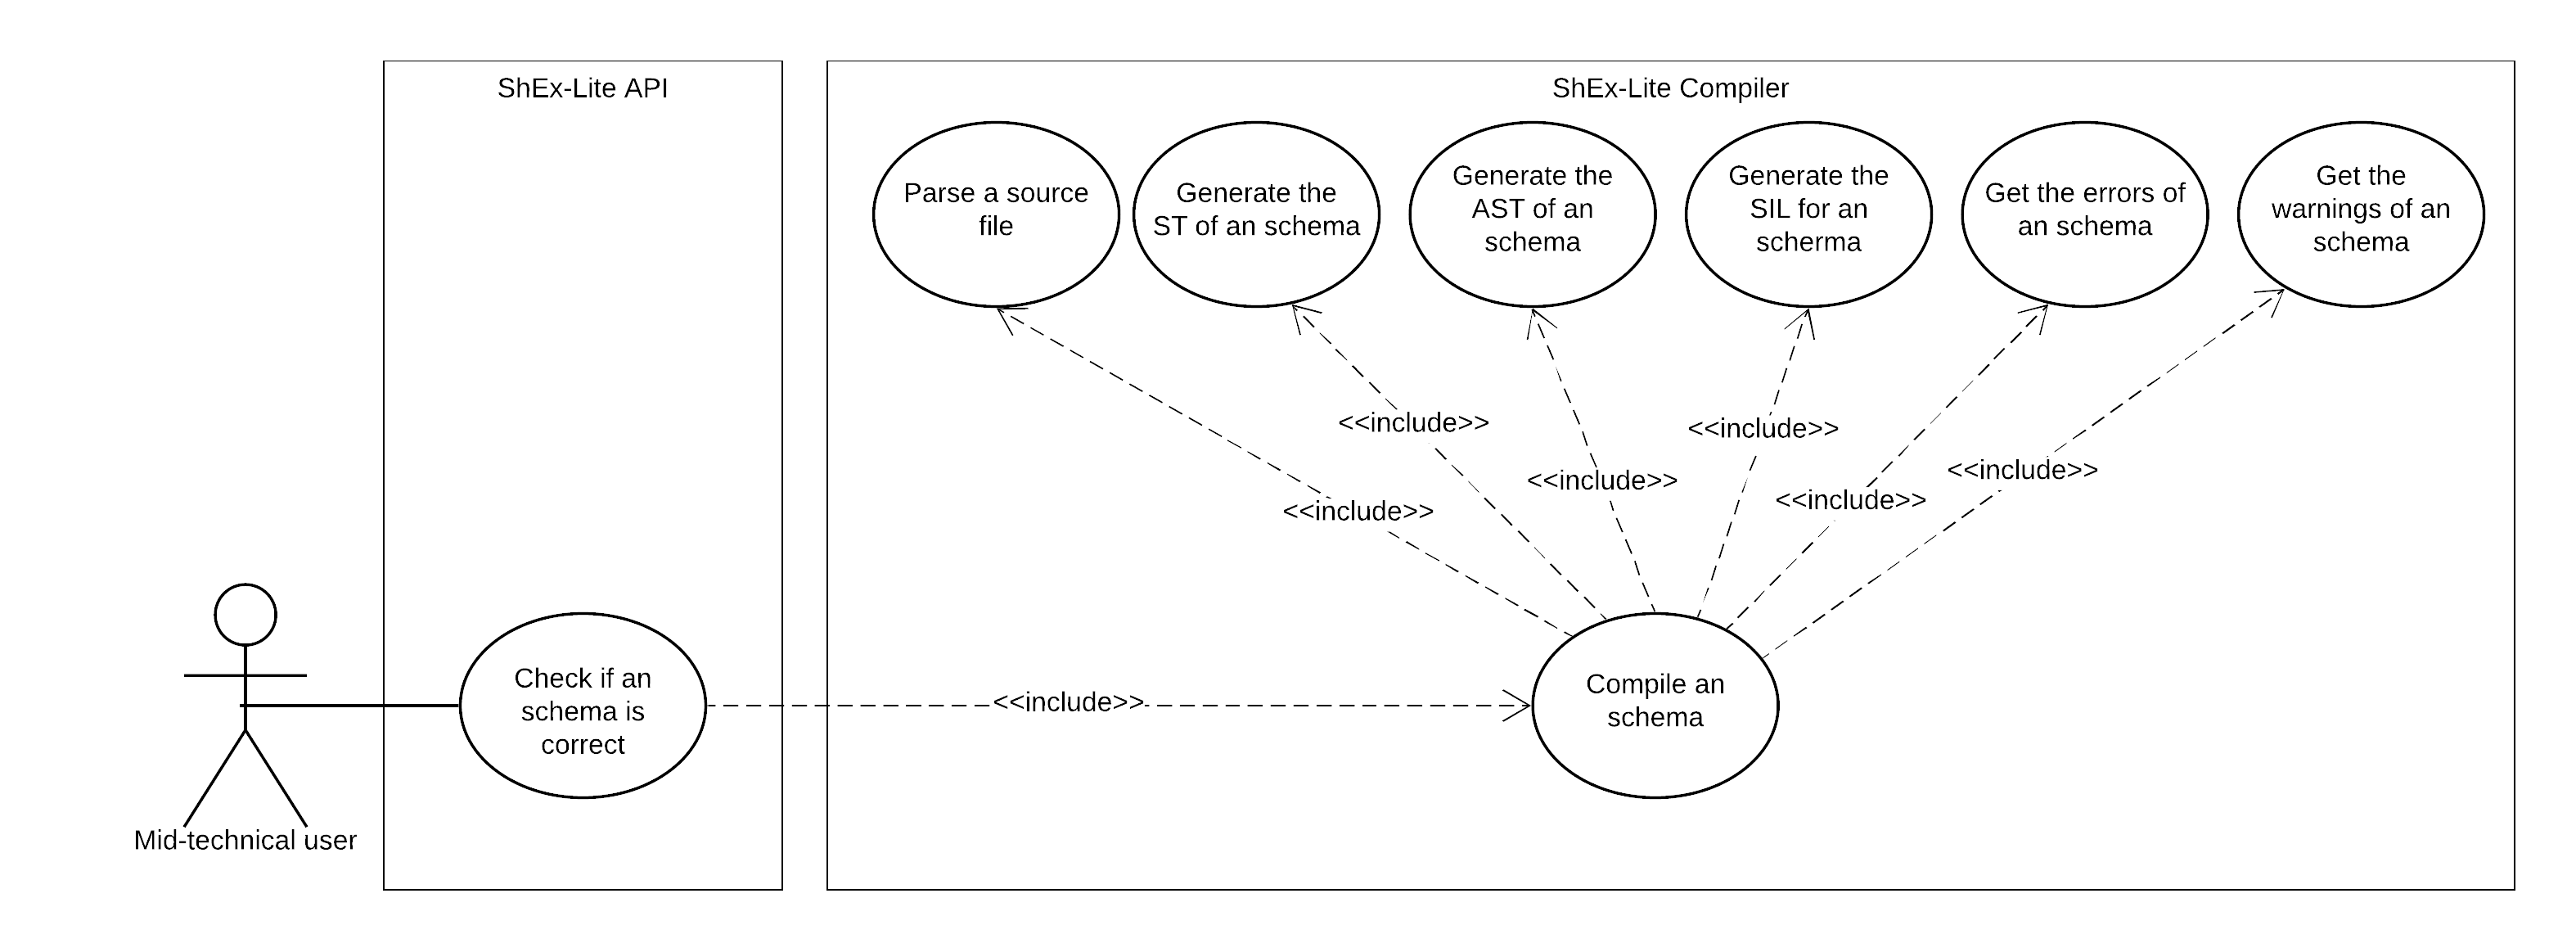
\includegraphics{shex-lite-use-case-mid-tech.png}
    \caption[Extension of the use case view for a mid technical user]{Extension of the use case view for a 
    mid technical user.}
    \labfig{shex-lite-use-cases-03}
\end{figure}

\begin{table}[h!]
    \begin{tabular}{ | m{2cm} | m{8cm}| }
        \hline
        Use Case Number & 2 \\
        \hline
        Description & Check if an schema is correct from the API. \\
        \hline
        Actor & Mid technical user. \\
        \hline
        Flow & The actor wants to check if schema is correct or not. If it is not correct wants to see all 
        the warnings / errors. For this purpose the actor introduces the schema in the API and starts 
        the flow. Once the flow is complete the actor wants to see information that helps to decide if the 
        schema is correct or not. \\
        \hline
    \end{tabular}
    \caption[Definition of the use case number 2 for the mid technical user]{Definition of the use case 
    number 2 for the mid technical user.}
    \labtab{use-case-02-tab}
\end{table}

\subsubsection{ShEx Developer}
Also from \reffig{shex-lite-use-cases-01} we see that the main use case for a ShEx Developer for the front-end
of the compiler is to integrate the different API components on other Java based applications. 

\begin{figure}[hb]
    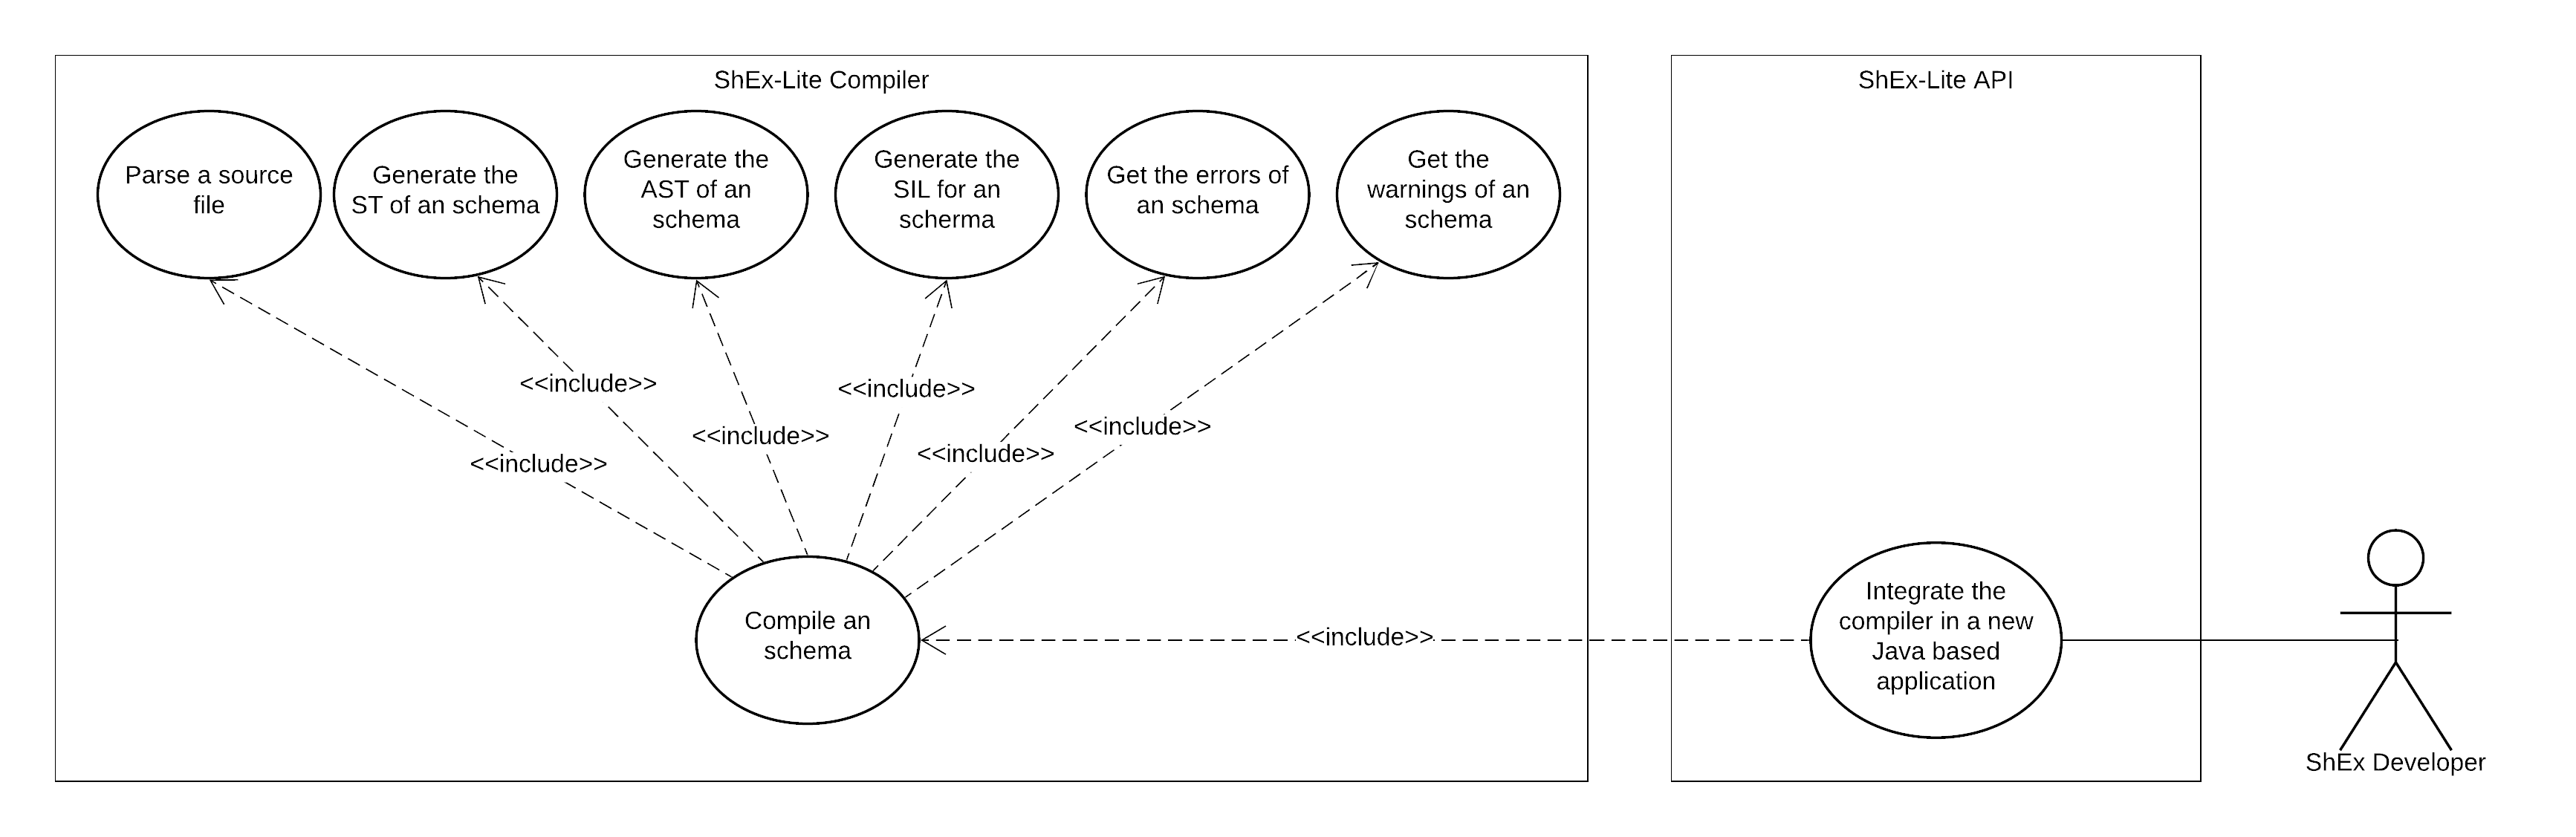
\includegraphics{shex-lite-use-case-dev.png}
    \caption[Extension of the use case view for a mid technical user]{Extension of the use case view for a 
    mid technical user.}
    \labfig{shex-lite-use-cases-04}
\end{figure}

\begin{table}
    \begin{tabular}{ | m{2cm} | m{8cm}| }
        \toprule
        Use Case Number & 3 \\
        \midrule
        Description & Integrate the compiler in a new Java based application. \\
        \midrule
        Actor & ShEx developer. \\
        \midrule
        Flow & The actor wants to integrate the compiler in to a new java base application. For that purpose 
        the actor will use a public API that allow the actor to integrate the actions described in the use case 
        2. \\
        \bottomrule
    \end{tabular}
    \caption[Definition of the use case number 3 for the ShEx developer user]{Definition of the use case number 
    3 for the ShEx developer user.}
    \labtab{use-case-04-tab}
\end{table}

\bigskip
The previous use cases might seem like the system is really simple, but far from truth the
fact that the interface with the target users is simple does not define the complexity of the
system, as this, lives inside of it. In order to capture this complexity we will proceed now to
analyze the requirements that the implemented system must meet. 

\subsection{Requirements}
Once we have explored the use cases for the compiler we can capture the requirements that will lead
the design of the compiler.

\subsubsection{External interfaces}
These requirements affect to software and hardware communication interfaces.

\subsubsection{Functional Requirements}
Requirements related to the functions of the system.

\subsubsection{Performance Requirements}
These requirements are related to the load that the system should tolerate.

\subsubsection{System Attributes}
Quality attributes of the system, such as usability, accessibility...